\documentclass[11pt]{article}

\usepackage[paperwidth=13.6cm, paperheight=11cm, top=0cm]{geometry}
\usepackage{MinionPro}
\usepackage{tikz}
\usepackage[pscoord]{eso-pic}

\newcommand{\placetextbox}[3]{% 
  \setbox0=\hbox{#3}
  \AddToShipoutPictureFG*{%
    \put(\LenToUnit{#1\paperwidth},\LenToUnit{#2\paperheight}){\vtop{{\null}\makebox[0pt][l]{#3}}}%
  }
}

\newcommand{\doortitle}[1]{\centering \Huge #1}

% \student{<column number (1 or 2)>}{<row number (1, 2, 3 or 4)>}{<name>}{<path to image>}
\newcommand{\student}[4]{%
	\placetextbox{\column{#1}}{\studentrow{#2}}{\hspace{0.7cm}\Large #3}
	\placetextbox{\column{#1}}{\studentrow{#2}}{\hspace*{-1cm}\includegraphics[width=1.6cm, height=1.6cm]{#4}}
}

\newcommand{\column}[1]{%
	\ifnum#1=1
		0.095
	\fi
	\ifnum#1=2
		0.595
	\fi
}

\newcommand{\studentrow}[1]{%
	\ifnum#1=1
		0.8
	\fi
	\ifnum#1=2
		0.6
	\fi
	\ifnum#1=3
		0.4
	\fi
	\ifnum#1=4
		0.2
	\fi
}

\pagenumbering{gobble}

\begin{document}

\tikz[remember picture,overlay] \node[opacity=0.3,inner sep=0pt] at (current page.center){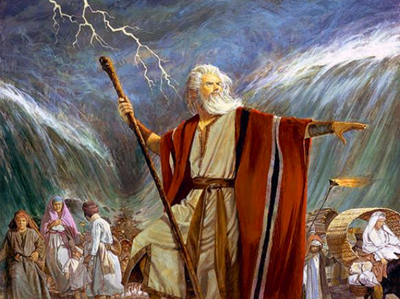
\includegraphics[width=\paperwidth,height=\paperheight]{background.png}};

\doortitle{PhD4 is \emph{The Bible}}

\student{1}{1}{J. `Lazarus' Walton}{lazarus.jpg}
\student{2}{1}{H. `Adam'  Alshammari}{adam.jpg}
\student{1}{2}{L. `The Snake' Dobson}{snake.jpg}
\student{2}{2}{C. `Holy Spirit' Evirgen}{spirit.jpg}
\student{1}{3}{L. `The Donkey' Wadkin}{donkey.png}
\student{2}{3}{A. `Gabriel' Hindle}{angel.jpg}
\student{1}{4}{R. `Judas' Ratnasingam}{judas.jpg}
\student{2}{4}{J. `The Apple' Hollins}{apple.jpg}

\end{document}
